%%%%%%%%%%%%%%%%%%%%%%%%%%%%%%%%%%%%%%%%%%%%%%%%%%%%%%%%%%%%%%%%%%%%%%%%%%%%%%
%
% Main content starts here
%
%%%%%%%%%%%%%%%%%%%%%%%%%%%%%%%%%%%%%%%%%%%%%%%%%%%%%%%%%%%%%%%%%%%%%%%%%%%%%%


\chapter{Introduction}
\label{sec:introduction}



\section{Problem statement}
\section{Thesis organization and contributions}

The thesis is organized as follows:
\begin{itemize}

\item[] \emph{Chapter 2:} 
\\We further continue with the theoretical part, such as .


\item[] \emph{Chapter 3:}
\\This chapter gives an overview of the state of the art of research in 


\item[] \emph{Chapter 4:} 
\\In this chapter, we are moving into the main part of the thesis - the implementation of the described approach. Additionally, the chapter presents the results of the experiments that were made. Furthermore, we evaluate and discuss the results of the experimental part of the approach.

\item[] \emph{Chapter 5:} 
\\This chapter is devoted to applications  We also discuss possible future work and collaboration with another university group of students.

\item[] \emph{Chapter 6:} 
\\We summarize the finding of  this thesis in this chapter, review the results and discuss possible tasks for future work.

\end{itemize}


In this thesis, the following contributions are made:
\begin{enumerate}

\item We propose a similarity search approach 

\item  W....

\item  We analyze the results and performance from the experimental part of the ....

\end{enumerate}







% First Paragraph
% CORE MESSAGE OF THIS PARAGRAPH:
\todo{P1.1. What is the large scope of the problem?}
\todo{P1.2. What is the specific problem?}

% Second Paragraph
% CORE MESSAGE OF THIS PARAGRAPH:
\todo{P2.1. The second paragraph should be about what have others been doing}
\todo{P2.2. Why is the problem important? Why was this work carried out?}

% Third Paragraph
% CORE MESSAGE OF THIS PARAGRAPH:
\todo{P3.1. What have you done?}
\todo{P3.2. What is new about your work?}

% Fourth paragraph
% CORE MESSAGE OF THIS PARAGRAPH:
\todo{P4.1. What did you find out? What are the concrete results?}
\todo{P4.2. What are the implications? What does this mean for the bigger picture?}

LaTeX hints are provided in \autoref{chap:latexhints}.

\chapter{Literature Review}
In this chapter, we present the theoretical background of the basic concepts of the thesis. Moreover, we define and explain different methods and algorithms that are used. 


\section{Quality}

\section{Quality models}

\subsection{Quality model ISO 9126-1}
text text
e

de
de
de

\begin{table}[h!]
    \caption{Sub-characteristics of the ISO 9126-1 quality modeL.}
	\begin{tabularx}{\textwidth}{X | X }
		%\hline
	    \textbf{Quality Characteristics} & \textbf{Sub-characteristics}	
	    \\ \hline
		\\ %\hline
		Functionality
        & Suitability
        
        Accuracy
        
        Interoperability 
        
        Security
        
        Compliance			 
		
		\\ \hline
	     \\ %\hline
		Reliability    
        
        &  Maturity 
        
        Fault tolerance 
        
        Recoverability 
        
        Compliance
		
		\\ \hline
	     \\ %\hline
	    Usability       
        
        & Understandability 
        
        Learnability 
        
        Operability 
        
        Compliance
    
	    \\ \hline
	  \\ %\hline
	   Efficiency &  Time behavior 
        
        Resource behavior 
        
        Compliance    
        \\ %\hline
	    \\ \hline
	    \\ %\hline
	    
	   Maintainability	
       
       & Analyzability 
        
        Changeability 
        
        Stability 
        
        Testability 
        
        Compliance
        
	    \\ \hline
	    \\ %\hline
	    
	   Portability	
       
       & Adaptability
       
       Installability 
       
       Co-existence
       
       Replaceability 
       
       Compliance
        	   
	\end{tabularx}
	\label{tab:table1}
	
\end{table}


\subsection{Quality model ISO 25010? }



\begin{table}[h!]
    \caption{Sub-characteristics of the Quality model-ISO/IEC 25010}
	\begin{tabularx}{\textwidth}{X | X }
		%\hline
	    \textbf{Quality Characteristics} & \textbf{Sub-characteristics}	
	    \\ \hline
		\\ %\hline
		Functional Suitability
       
        & Functional completeness
        
        Functional correctness
        
        Functional appropriateness		
        
        \\ %\hline
		\\ \hline
	     \\ %\hline
		Reliability    
        
        &  Maturity 
        
        Availability
        
        Fault tolerance
        
        Recoverability
        
		\\ \hline
	     \\ %\hline
	    Performance efficiency       
        
        & Time behaviour
        
        Resource utilization
        
        Capacity
        
        
	    \\ \hline
	  \\ %\hline
	   Compatibility  
       
       &  Co-existence
       
       Interoperability   
       
     
	    \\ \hline
	    \\ %\hline
	    
	   Usability	
       
       & Appropriateness recognizability
       
       Learnability
       
       Operability
       
       User error protection
       
       User interface aesthetics

       Accessibility
       
      
	    \\ \hline
	    \\ %\hline
	    
	   Security	
       
       & Confidentiality
       
       Integrity
       
       Non-repudiation
       
       Accountability
       
       Authenticity
              
       
	    \\ \hline
	    \\ %\hline
	    
	   Maintainability	
       
       &  Modularity
       
       Reusability
       
       Analysability
       
       Modifiability
       
       Testability
     
	    \\ \hline
	    \\ %\hline
	    
	   Portability	
       
       & Adaptability
       
       Installability
       
       Replaceability
        	   
	\end{tabularx}
	\label{tab:table1}
	
\end{table}

\section{Cognitive Load Theory (CLT)}

\section{Theory of Program Comprehension}
Describe relevant scientific literature related 


\section{Studies using Eye Tracking}


In this chapter, we present different works about topics, that are similar to the topic of this thesis. More specifically, we present literature, which discusses different approaches that are used in order to 


\begin{figure}
  \centering
  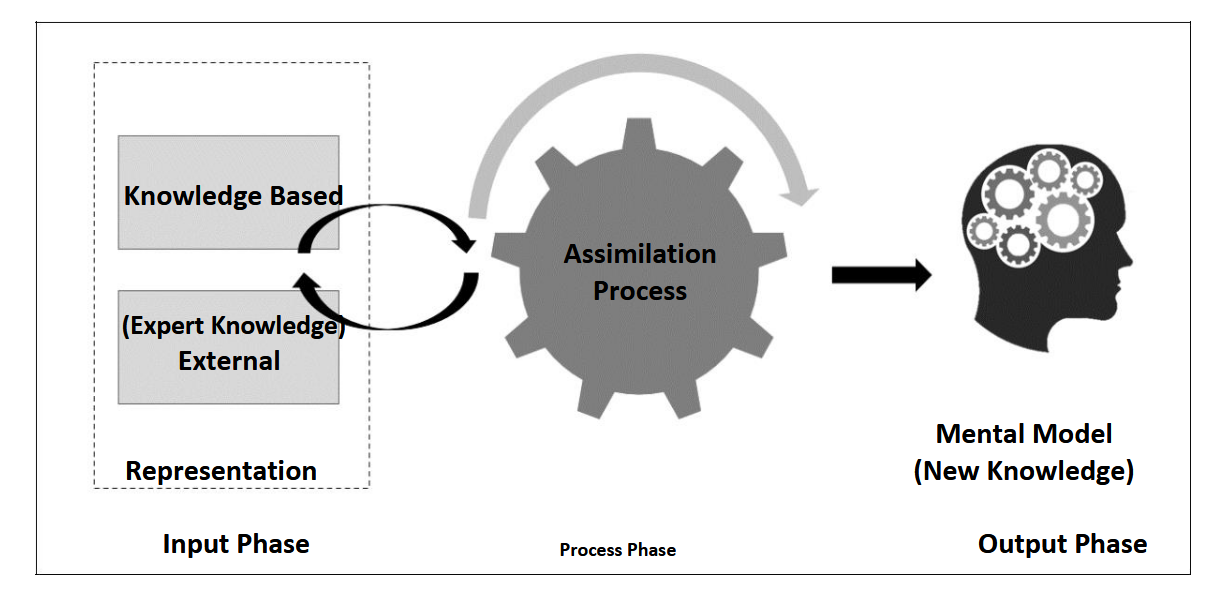
\includegraphics[width=\textwidth]{figures/program_Comprehension_Process.png}
  \caption{The Program Comprehension Process}
  \label{fig:AnhangsChor}
\end{figure}



\chapter{Study Design}

\section{Methodology}

\section{Procedure}

\section{Measurements}

\section{Participants}

\chapter{Results}

\chapter{Discussion - Interpretation of Results}

\chapter{Conclusion and Outlook}
\label{sec:conclusion}
